\documentclass{beamer}
\usepackage[italian]{babel}

\usepackage{caption}
\usepackage{listings}

\usepackage{multicol}
\usepackage{copyrightbox}
\usepackage{bookmark}
\usepackage{tikz}
\usetikzlibrary{arrows.meta}

\usepackage[backend=bibtex,style=authortitle]{biblatex}
\addbibresource{bibliografy.bib}

\usepackage{minted}
\setminted{fontsize=\small}

\usepackage{subfigure}

\definecolor{green(html/cssgreen)}{rgb}{0.0, 0.5, 0.0}

\usetheme{Pittsburgh}
\usefonttheme{serif}
\setbeamerfont{caption}{size=\tiny}
\setbeamertemplate{navigation symbols}{}
\setbeamertemplate{caption}{\raggedright\insertcaption\par}
\setbeamertemplate{footline}[frame number]
\setbeamertemplate{frametitle}{
    \vspace{20pt}
    \begin{centering}
        \insertframetitle\\
    \end{centering}
    \vspace{-20pt}
}

\title{Elm in Practice: Features and Trade-Offs of a Functional Language for the Web}
\author{Davide Cioni}
\author[Davide Cioni]{
    Davide Cioni
    \\{\small Relatore: Chiar.mo Prof. Saverio Giallorenzo}
    }
\institute{Alma Mater Studiorum $\cdot$ Università di Bologna}
\date{18 Dicembre 2024}

\begin{document}

\begin{frame}
  \titlepage
\end{frame}

\begin{frame}
    \frametitle{Perché Elm? JavaScript}
    \begin{figure}
      \centering
      
\includegraphics[height=100pt]{assets/js-logo.png}
    \end{figure}
    \begin{itemize}
        \item Linguaggio dinamicamente tipato
        \item Multi-paradigma
        \item Fragile per codebase di dimensioni significative
    \end{itemize}
\end{frame}

\begin{frame}
  \frametitle{Elm}
  \begin{figure}
    \centering
    
\includegraphics[height=100pt]{assets/elm-logo.png}
  \end{figure}
  \begin{itemize}
      \item Linguaggio staticamente tipato
      \item Puramente funzionale
      \item Interoperabilità limitata con JavaScript
  \end{itemize}
\end{frame}


\begin{frame}
  \frametitle{Design goals}
  \begin{figure}
    \centering
    
\includegraphics[height=100pt]{assets/elm-logo.png}
  \end{figure}
  \begin{itemize}
      \item Errori a runtime estremamente rari
      \item Prevedibilità
      \item Semplice da usare e imparare
  \end{itemize}
\end{frame}

\begin{frame}[containsverbatim]
  \frametitle{The Elm Architecture}
  \begin{figure}
    \centering
    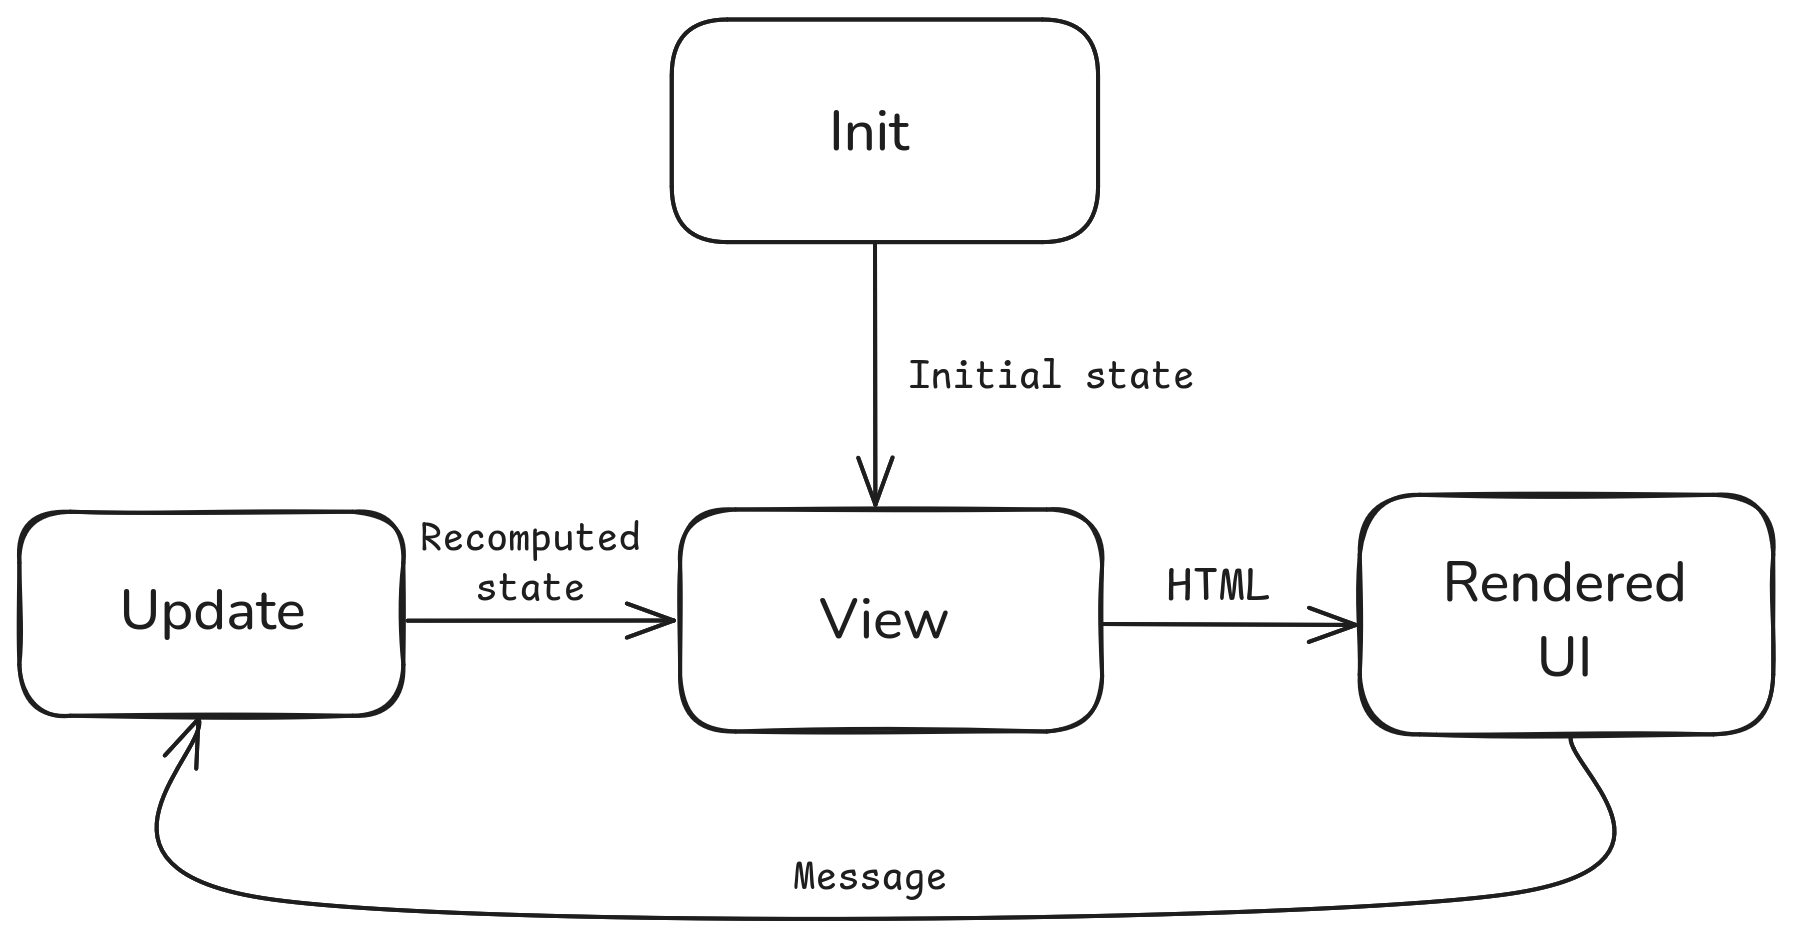
\includegraphics[height=125pt]{assets/elm-architecture.png}
  \end{figure}
  \begin{itemize}
      \item\begin{minted}{elm}
type Model = ...
      \end{minted}
      \item\begin{minted}{elm}
view : Model -> Html Msg
      \end{minted}
      \item\begin{minted}{elm}
update : Msg -> Model -> Model
      \end{minted}
  \end{itemize}

\end{frame}

\begin{frame}
  \frametitle{Architettura senza componenti}
  La Elm Architecture non supporta componenti dotato di stato locale.\\

  Il \texttt{Model} deve avere accesso a ogni parte dello stato, indipendentemente dalla posizione nel tree in cui questo viene effettivamente usato.
\end{frame}

\begin{frame}
  \frametitle{Interoperabilità}
  Non è possibile chiamare direttamente funzioni JavaScript da Elm e usare i valori di ritorno, in quanto nessuna forma di FFI è supportata.\\

  Sono invece presenti due metodi per interoperare con JavaScript:
  \vspace{3pt}
  \begin{itemize}
    \item Porte
    \item Web Components
  \end{itemize}

\end{frame}

\begin{frame}[containsverbatim]
  \frametitle{Commands and Subsctiptions}
  \begin{figure}
    \centering
    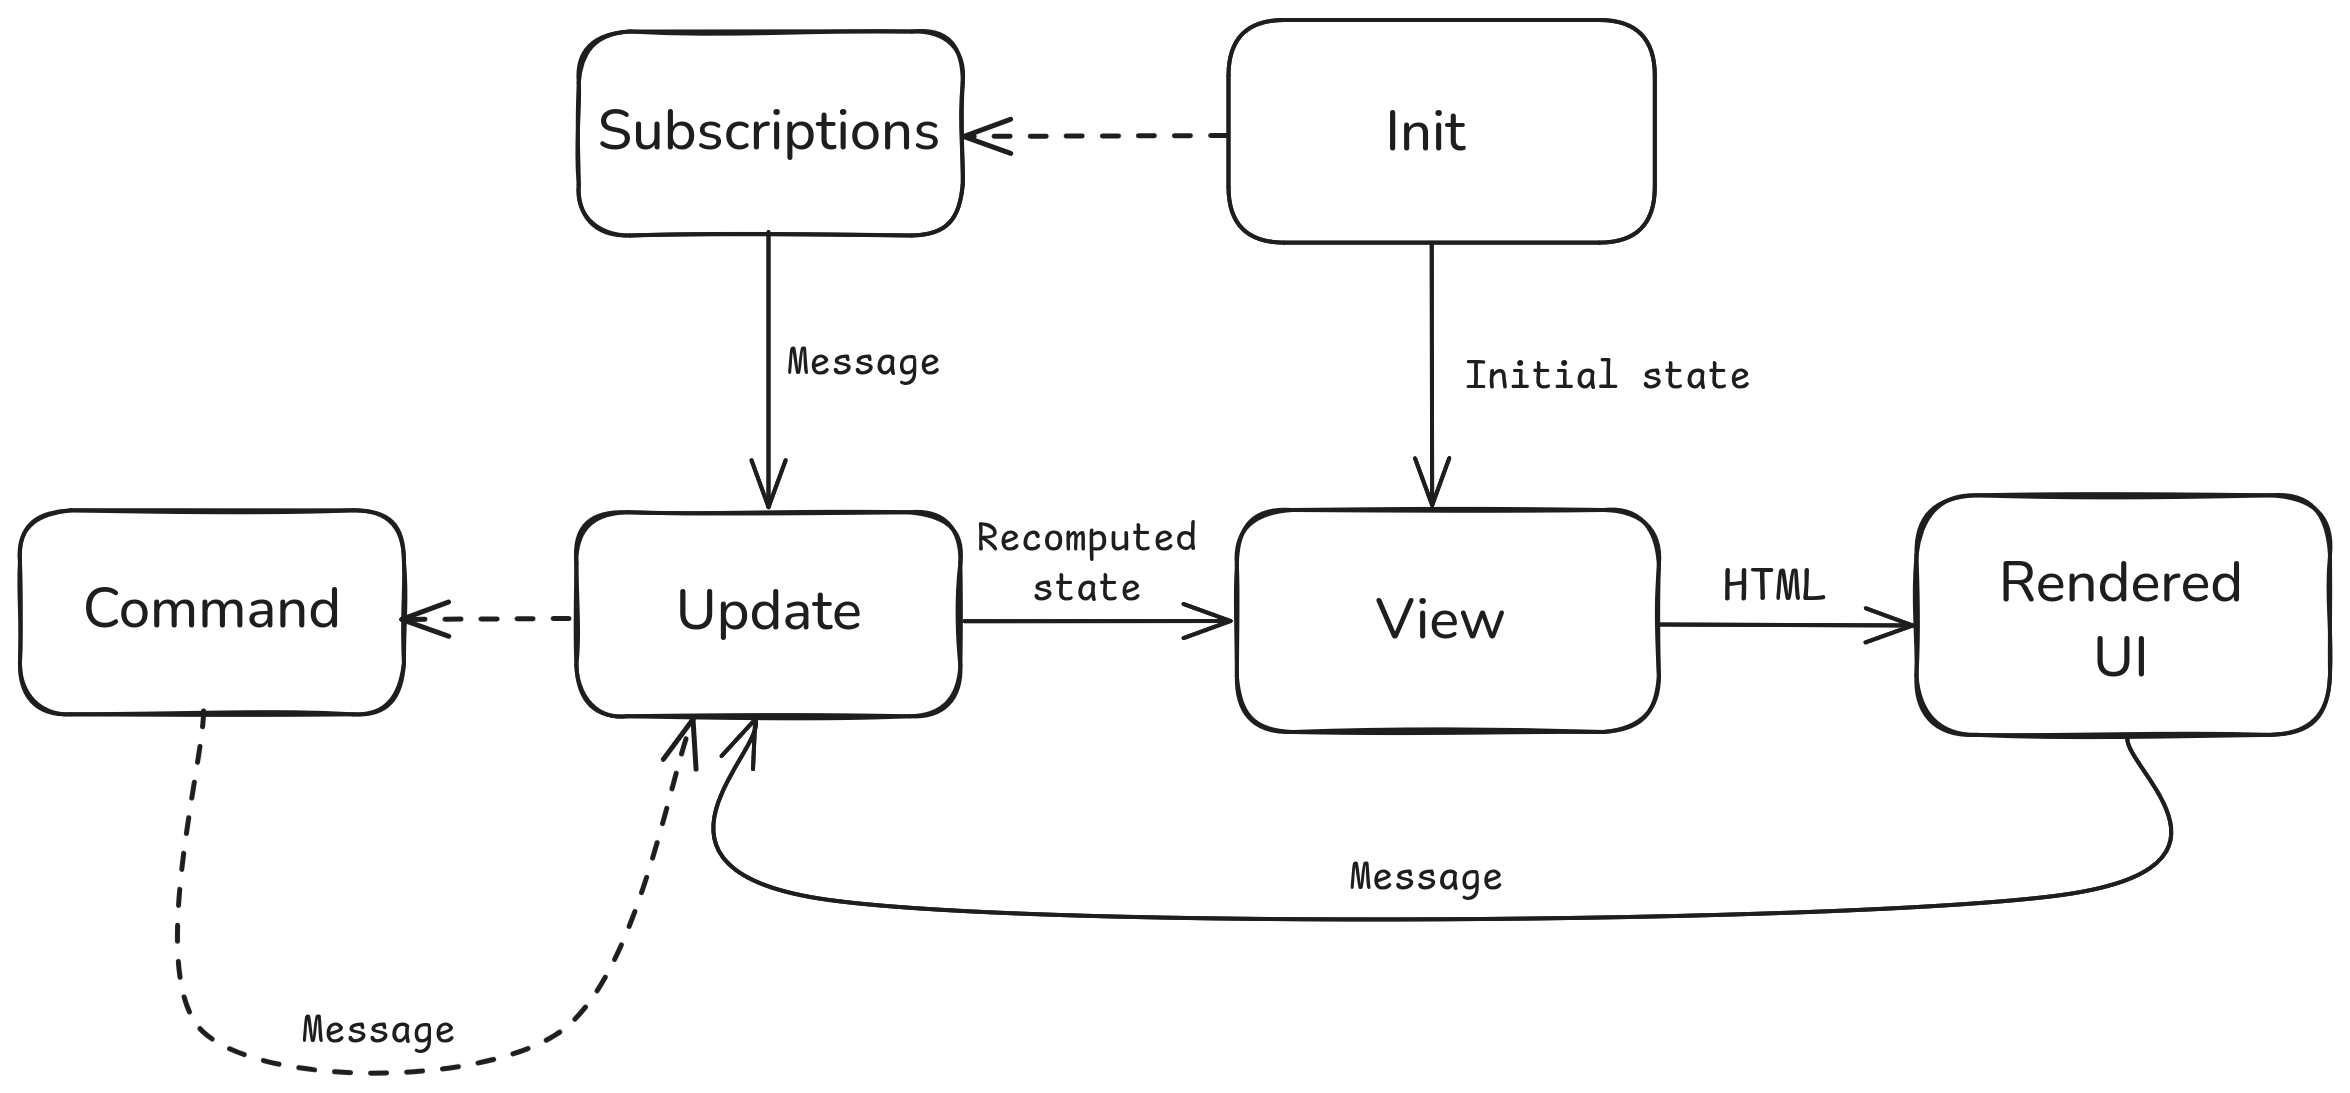
\includegraphics[height=150pt]{assets/elm-architecture-xt.png}
  \end{figure}
  \begin{itemize}
      \item\begin{minted}{elm}
subscriptions : Model -> Sub Msg
      \end{minted}
      \item\begin{minted}{elm}
update : Msg -> Model -> ( Model, Cmd Msg )
      \end{minted}
  \end{itemize}

\end{frame}

\begin{frame}[containsverbatim]
  \frametitle{Porte}
  \textbf{Elm}
  \begin{minted}{elm}
port storeId : String -> Cmd msg
port removeId : () -> Cmd msg
port listenId : (Maybe String -> msg) -> Sub msg
  \end{minted}
  \vspace{10pt}
  \textbf{JavaScript}
  \begin{minted}{js}
app.ports.storeId.subscribe((id) => {...});
app.ports.removeId.subscribe((id) => {...});
app.ports.listenId.send(...);
  \end{minted}
\end{frame}

\begin{frame}
  \frametitle{Caratteristiche e Trade-Off}
  \begin{itemize}
    \item Runtime safety maggiore delle altre soluzioni
    \item Performance e asset size competitivi
    \item Architettura semplice ma solida ed espressiva
    \item Web Platform APIs non interamente supportate
    \item No FFI
    \item Impossibilità di incapsulare lo stato
  \end{itemize}
\end{frame}

\begin{frame}[plain]
  \vfill
  \centering
  \Huge Grazie dell'attenzione
  \vfill
\end{frame}

\end{document}
